\documentclass{article}
\usepackage[usenames,dvipsnames]{pstricks}
\usepackage{amsfonts}
\usepackage{amsmath}
\usepackage{amssymb}
\usepackage{epsfig}
\usepackage{graphicx}
\usepackage{mathrsfs}
\usepackage{pst-grad} % For gradients
\usepackage{pst-plot} % For axes
\usepackage[justification=centering]{caption}
\usepackage{subcaption}
\usepackage{tikz}
\usepackage{fancyhdr}
\pagestyle{fancy}
\lhead{COMP 590}
\chead{Mark I. Edwards}
\rhead{Homework 3}

\title{COMP 590 Homework 3}
\author{Mark I. Edwards}
\date{April 21, 2016}

\begin{document}
\maketitle
\section*{Problem 1}
I first prove that if $A$ is a matrix with eigenvalue $\lambda$ and eigenvector
$v$, then $\lambda^n$ is an eigenvalue of $A^n$ for positive integers $n$. 

I prove this via induction. Our base case is our initial assumption, so I
proceed to the induction step. I suppose that
\[ A^n v = \lambda^n v \]
And then show that
\[ A^{n+1} v = \lambda^{n+1} v \]
From our assumption, I left-multiply both sides by $A$, yielding
\[ AA^n v = A^{n+1}v = A \lambda^n v = \lambda^n Av \]
From our initial assumption, we know that 
\[ Av = \lambda v \]
thus
\[ A^{n+1} v = \lambda^n (\lambda v) = \lambda^{n+1} v \]
as required. 

With this in mind, I now turn to consider 
\[ \lim_{n \rightarrow \infty} \lambda^n \]
when 
\[ \lim_{n \rightarrow \infty} A^n \]
exists ($A^n$ does not approach infinity). We know that $ \lim_{n \rightarrow
\infty} \lambda^n $ exists, by right-multiplying both sides by $v$ and noting
the similarity to what we just proved. Now let $\lambda = a e^{i\theta}$ for
some real $a$ and $\theta$. There are now 3 possibilities: 
\begin{align*}
|a| <& 1 \\
|a| =& 1 \\
|a| >& 1 
\end{align*}
Now if $|a| < 1$, $\lambda^n \rightarrow 0$. If $|a|=1$, then $ae^{in\theta} =
\lambda^n$ will only converge if $\theta = 0$, since otherwise $\lambda^n$ will
continuously traverse the edge of the unit circle. If $|a| > 1$, $|\lambda^n| =
|a|^n$ will grow infinitely as $n$ increases, and so $\lambda^n$ will not
converge. In summary, $\lambda$ will only converge if $|\lambda| < 1$ or
$\lambda = \pm 1$. 

As stated in class, $A = e^{-L(D)}$ contains a rooted out branching if and only
if the agreement algorithm converges. As of such, we know that the eigenvalues
$A$ are either $\pm 1$ or have magnitude less than 1, because the agreement
algorithm can then be written as $x(t) = x_0 A^t$. 

\section*{Problem 2}
In order to analyze this, let us consider the discrete time agreement algorithm.
\[ z(k+1) = e^{-\delta L(D)}z(k) \]
As noted on page 74 of Mesbahi and Egerstedt. And as noted by Corollary 4.2 of
the same book, the digraph $D$ is rooted out branching if and only if one of the
columns of $e^{-\delta L(D)}$ is positive. From this, we can see that if the
digraph $D$ is rooted out branching, 
\[ V(z(k+1)) < V(z(k)) \]
because each time step $k$ updates the $z$ value by taking a convex combination
of itself and the other vertex values, and because one column of $e^{-\delta
L(D)}$ is positive. This means that the maximum and minimum values approach one
another since they are ``connected'' by that positive column, representing some
connection within the digraph. This assumes that the minimum and maximum values
are different, of course, but if they are the same then we are already in the
agreement subspace. 

I show this in effect for the directed graph in Figure 1. 
\begin{figure}[h!]
\centering
\caption{A 5 Node Directed Rooted Out Branching Graph}
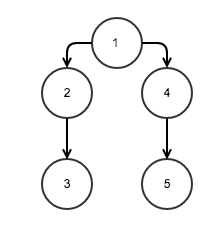
\includegraphics[width=0.3\textwidth]{p2graph.png}
\end{figure}
With adjacency matrix
\[ \begin{bmatrix}
     0  &  0   & 0   & 0  &  0\\
     1  &  0  &  0  &  0  &  0\\
     0  &  1  &  0  &  0  &  0\\
     1  &  0  &  0  &  0  &  0\\
     0  &  0  &  0  &  1  &  0
\end{bmatrix}\]
And degree matrix
\[ \begin{bmatrix}
     0  &  0  &  0  &  0  &  0\\
     0  &  1  &  0  &  0  &  0\\
     0  &  0  &  1  &  0  &  0\\
     0  &  0  &  0  &  1  &  0\\
     0  &  0  &  0  &  0  &  1
\end{bmatrix} \]
Which yields the Laplacian
\[ -L = \begin{bmatrix}
     0  &  0  &  0  &  0  &  0\\
     1  & -1  &  0  &  0  &  0\\
     0  &  1  & -1  &  0  &  0\\
     1  &  0  &  0  & -1  &  0\\
     0  &  0  &  0  &  1  & -1
\end{bmatrix} \]
with initial values
\[ \begin{bmatrix}
    50\\
    30\\
    45\\
    70\\
    90
\end{bmatrix} \]
I implement the algorithm in \texttt{p2.m} and get the Lyapunov function using
\begin{verbatim}
max(vals) - min(vals)
\end{verbatim}
When plotted, this yields
\begin{figure}[h!]
\centering
\caption{Lyapunov Function}
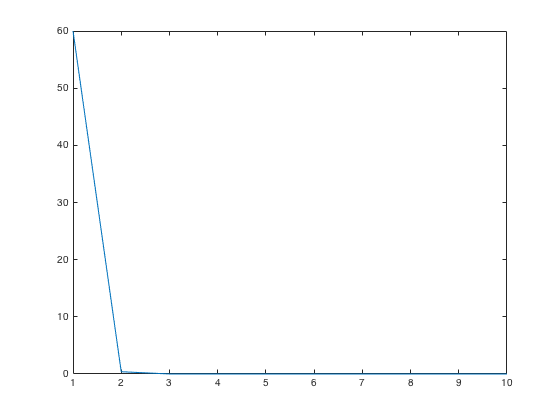
\includegraphics[width=0.5\textwidth]{p2plot.png}
\end{figure}

\section*{Problem 3}
Before I address the key issue of this problem, I would like to bring up the
small angle approximation which says that 
\[ \theta \approx \sin \theta \]
for small angles $\theta$. This is very closely related to the issue of
convergence of this algorithm, because the failure of this approximation for
larger angles results in the failure of the algorithm when the differences
between the values of neighboring vertices is sufficiently large.
\begin{figure}[h!]
\centering
\caption{Absolute Error of the Small Angle Approximation}
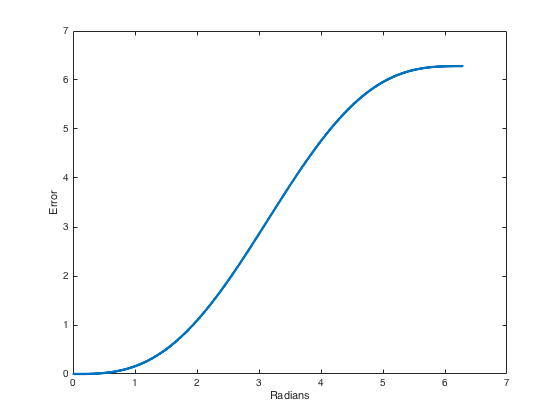
\includegraphics[width=0.5\textwidth]{saa-error.png}
\end{figure}
The following
figures were generated by varying values in the code in \texttt{hw3\_problem3.m}
which calls the function that implements the algorithm in \texttt{p3.m}. The
code in \texttt{hw3\_problem3.m} generates connected graphs with 5 nodes and
gradually adds edges until the graph is fully connected. In the case that the
algorithm does not converge, \texttt{p3.m} will automatically exit after
$10^{5}$ steps. All graphs have exactly 5 nodes, but varying numbers of edges. 

\begin{figure}[h!]
\caption{Initial Values Between ($-\pi$ to $\pi$)}
\centering
\begin{subfigure}[t]{0.3\textwidth}
\centering
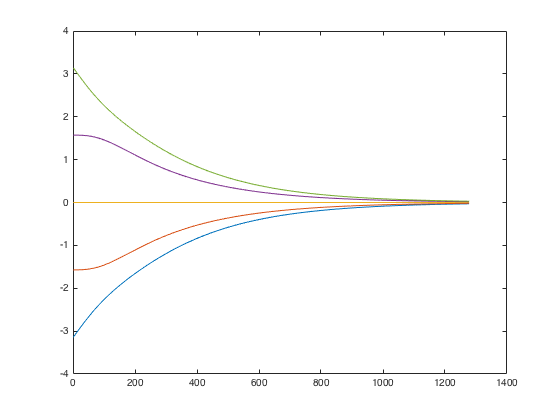
\includegraphics[width=\textwidth]{./p3minimally_connected.png}
\caption{A Path From 1 to 5}
\end{subfigure}
\begin{subfigure}[t]{0.3\textwidth}
\centering
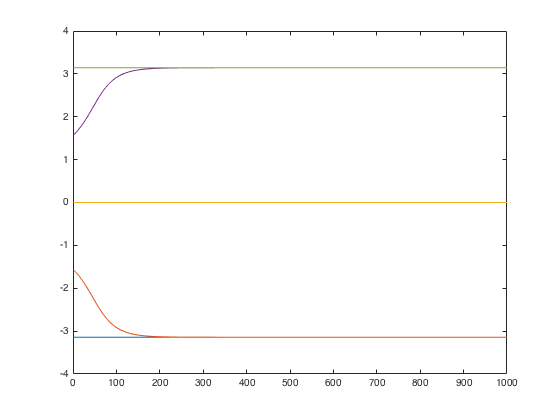
\includegraphics[width=\textwidth]{p3_maximally_connected.png}
\caption{A Fully Connected Graph}
\end{subfigure}
\begin{subfigure}[t]{0.3\textwidth}
\centering
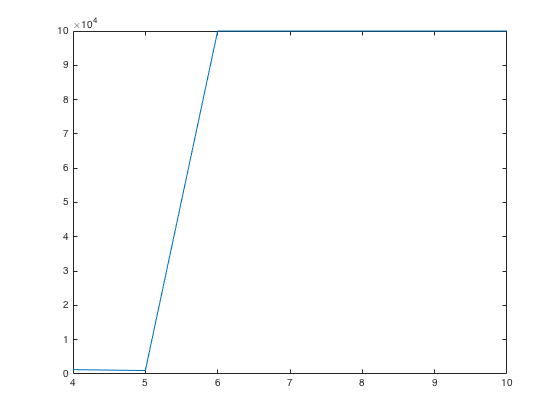
\includegraphics[width=\textwidth]{p3_convergence_steps.png}
\caption{Number of Steps vs Edges}
\end{subfigure}
\end{figure}
From Figure 4(b) we can see an example of an initial set up that does not
converge. In fact, as shown in Figure 4(c), applying the algorithm to all of the
graphs in my progression (of sequentially adding edges) will diverge for all
graphs with more than 5 edges. Furthermore, while impossible to see clearly due
to the size of the figures, the graph with 5 edges converges faster than the one
with 4. 
\begin{figure}[h!]
\caption{Initial Values Between ($-\pi/2$ to $\pi/2$)}
\centering
\begin{subfigure}[t]{0.3\textwidth}
\centering
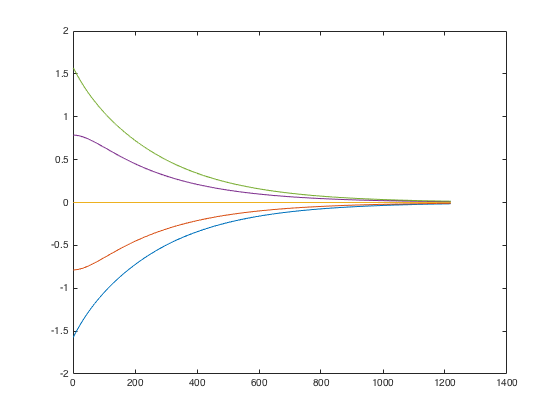
\includegraphics[width=\textwidth]{./pi-ov2-min.png}
\caption{A Path From 1 to 5}
\end{subfigure}
\begin{subfigure}[t]{0.3\textwidth}
\centering
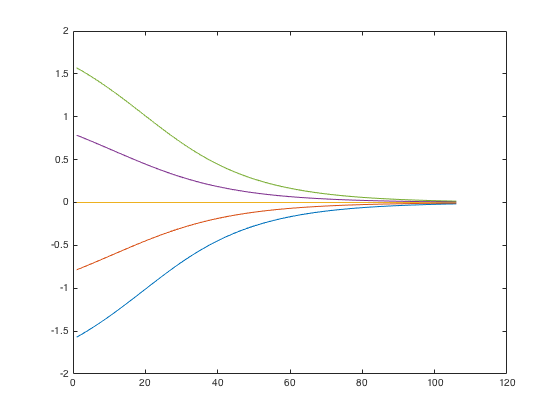
\includegraphics[width=\textwidth]{pi-ov2-max.png}
\caption{A Fully Connected Graph}
\end{subfigure}
\begin{subfigure}[t]{0.3\textwidth}
\centering
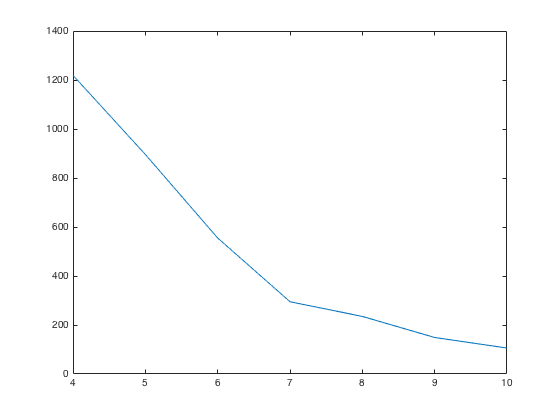
\includegraphics[width=\textwidth]{pi-ov2-conv.png}
\caption{Number of Steps vs Edges}
\end{subfigure}
\end{figure}

However, when we limit the range of initial $\theta$ values to $-\pi/2$ to
$\pi/2$, the algorithm converges quite quickly, as seen in Figure 5. From our
Assignment 1, we found that the standard agreement protocol with similar initial
values could take upward of a thousand iterations with similar step size on a
fully connected graph, while this algorithm takes just over 100. Furthermore,
now that every graph generated by the progression converges, we see the expected
decrease in the number of required steps as the number of edges increases. 
\begin{figure}[h!]
\caption{Initial Values Between ($-\pi$ to $\pi$)\\Omega between
$(\pi\cdot 0.9,-\pi\cdot 0.9)$}
\centering
\begin{subfigure}[t]{0.3\textwidth}
\centering
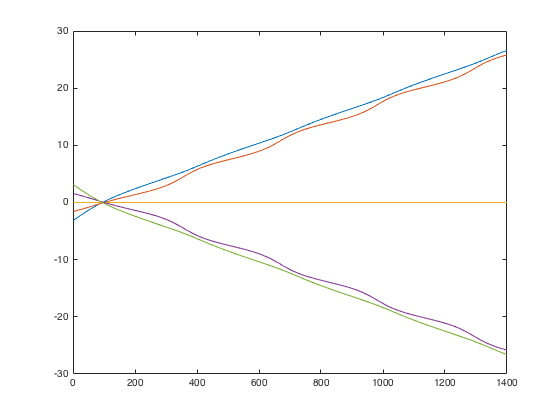
\includegraphics[width=\textwidth]{./pi-min-om0-9.png}
\caption{A Path From 1 to 5}
\end{subfigure}
\begin{subfigure}[t]{0.3\textwidth}
\centering
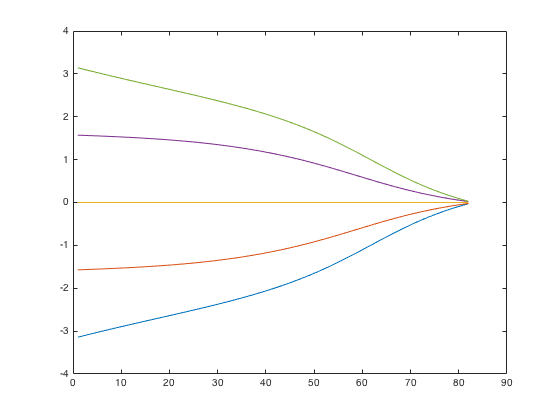
\includegraphics[width=\textwidth]{pi-om0-9-max.png}
\caption{A Fully Connected Graph}
\end{subfigure}
\begin{subfigure}[t]{0.3\textwidth}
\centering
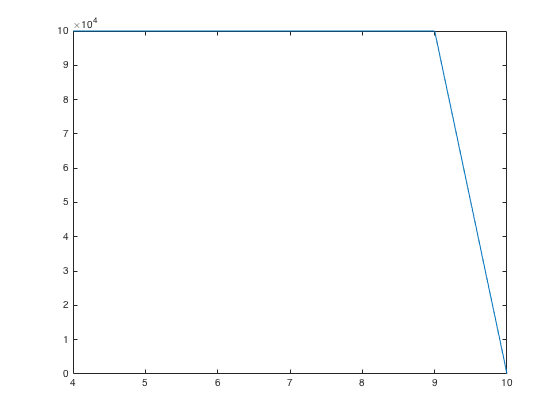
\includegraphics[width=\textwidth]{pi-om0-9-conv.png}
\caption{Number of Steps vs Edges}
\end{subfigure}
\end{figure}

Generally, random values of $\omega_i$ will not improve convergence. However, it
is possible to use $\omega$ to try to improve convergence by ``nudging'' the
values in the right direction. In Figure 6, we see the same set up as Figure 4
with the addition of an $\omega$ value that represents a bias representing
prior knowledge of the average of the other points. This is a powerful method to
try to achieve convergence with this algorithm when it would otherwise be
impossible, but it certainly isn't infallible. In Figure 6(a) we that the values
approach convergence, but then ``miss their mark'' and diverge. 
\begin{figure}[h!]
\centering
\caption{Initial Values Between ($-\pi$ to $\pi$)\\
Omega between $(\pi\cdot 0.9,-\pi\cdot 0.9)$\\Convergence Criterion Relaxed}
\begin{subfigure}[t]{0.3\textwidth}
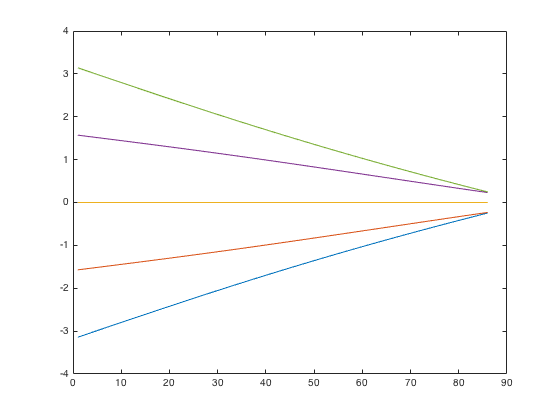
\includegraphics[width=\textwidth]{./pi-om0-9-min-rel.png}
\centering
\caption{A Path From 1 to 5}
\end{subfigure}
\begin{subfigure}[t]{0.3\textwidth}
\centering
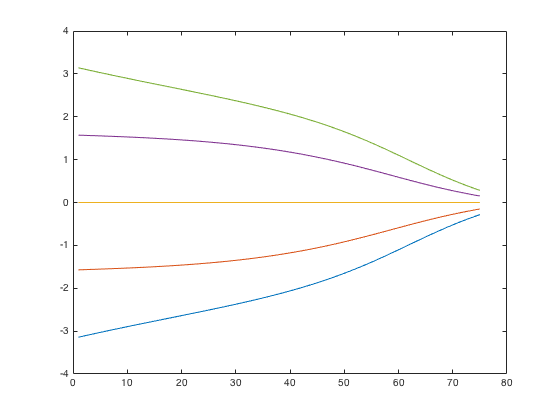
\includegraphics[width=\textwidth]{pi-om0-9-max-rel.png}
\caption{A Fully Connected Graph}
\end{subfigure}
\begin{subfigure}[t]{0.3\textwidth}
\centering
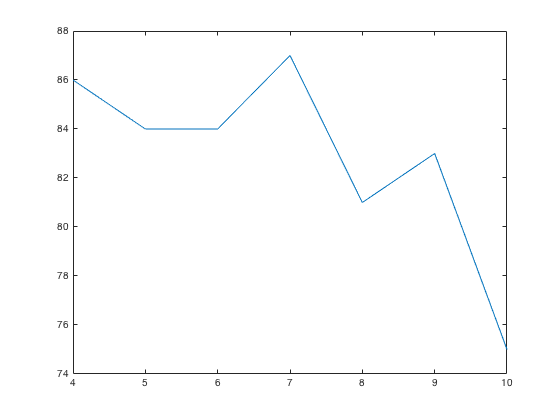
\includegraphics[width=\textwidth]{pi-om0-9-conv-rel.png}
\caption{Number of Steps vs Edges}
\end{subfigure}
\end{figure}
This can be adjusted for by relaxing the convergence criterion. In Figure 7, I
relax the convergence criterion from a 1\% difference from the mean to a 10\%
difference. This allows all the graphs in the progression to converge, and in
Figure 7(c) we see the expected reduction in convergence steps with respect to
increasing in connectivity, although the curve is now a jagged one. Generally,
relaxing the convergence criterion is necessary if we use $\omega$ to try to
improve convergence. In Figure 8 below, we see that adding an $\omega$ value to
the setup from Figure 5 causes the algorithm to diverge for most graphs in the
progression, following the pattern seen in Figure 8(a). 
\begin{figure}[h!]
\caption{Initial Values Between ($-\pi/2$ to $\pi/2$)\\Omega between
$(\pi\cdot 0.3,-\pi\cdot 0.3)$}
\centering
\begin{subfigure}[t]{0.3\textwidth}
\centering
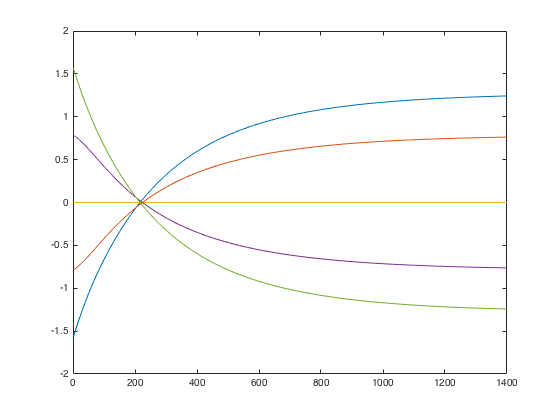
\includegraphics[width=\textwidth]{./pi-ov2-min-om0-3.png}
\caption{A Path From 1 to 5}
\end{subfigure}
\begin{subfigure}[t]{0.3\textwidth}
\centering
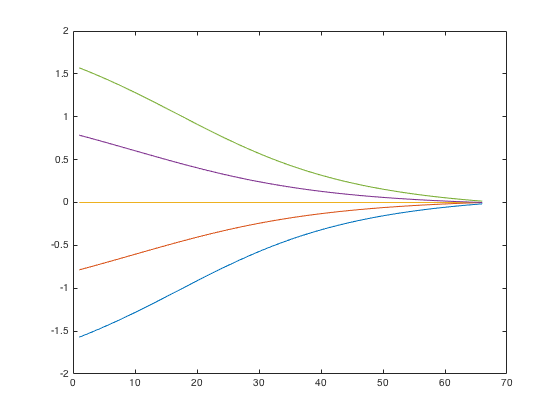
\includegraphics[width=\textwidth]{pi-ov2-max-om0-3.png}
\caption{A Fully Connected Graph}
\end{subfigure}
\begin{subfigure}[t]{0.3\textwidth}
\centering
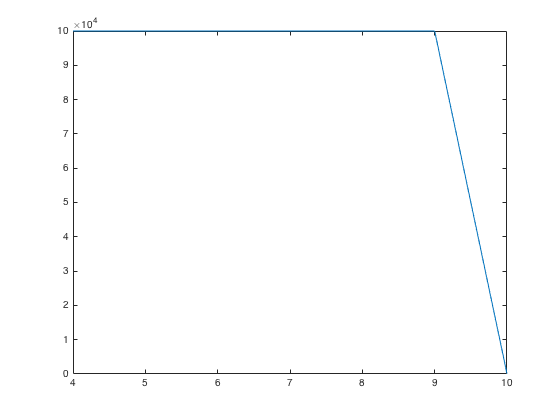
\includegraphics[width=\textwidth]{pi-ov2-om0-3-conv.png}
\caption{Number of Steps vs Edges}
\end{subfigure}
\end{figure}
Figure 8 shows that without relaxing the convergence condition, even graphs that
normally converge will diverge. 

In summary, this algorithm attempts to trade reliability for convergence speed.
Generally, convergence depends on the difference between the values of connected
nodes. This can be ``biased'' using the $\omega$ values, but using this often
requires that we relax our convergence criterion. 

\end{document}
